\chapter{Implementation}

The project is separated in two main components - the filter wrapper library and the user interface library.
Wrappers handle the application and parameters of each filter instance, while the UI handles the display
and interaction functionalities.

\section{Filter Wrapper Library}

Based on the OpenCV \verb|cv::Mat|, this library provides the means for applying a given filter on the input
frame, as well as a possibility to tweak the filters inherent parameters. The amount of filters supported can
be extended indefinitely, due to the use of a purely virtual abstract class, the \verb|GenericFilterWrapper|
class.

\begin{code}
	\caption{Generic wrapper class definition}
	\label{code:GenericFilterWrapper}
	\begin{lstlisting}
class GenericFilterWrapper {
    public:
        virtual void applyFilter(cv::Mat &inframe) = 0;
        virtual std::vector<parameterConfig> allParameterConfigs() = 0;
        virtual const char *filterName() = 0;
        virtual const char *filterDescription() = 0;
};
    \end{lstlisting}
\end{code}

As seen in \cref{code:GenericFilterWrapper}, the abstract class provides access to the function
applying the filter, as well as all details that can be shown in the user interface. For this reason,
the filter library can be used by any high-level graphical interface library, as long as a valid
\verb|cv::Mat| is provided. Initial prototypes were realized using the OpenCV HighUI library, and later
ported to the Qt Framework for the final product.

The class also provides access to a list of parameter configurations, that can be used in the user
interface to set up various tool-tips and interactive sliders.

\begin{code}
	\caption{Parameter configuration structure}
	\label{code:parameterConfig}
	\begin{lstlisting}
typedef struct _parameterConfig {
    const char* name;
    const char* description;
    int currentValue;
    int minValue;
    int maxValue;
    int step;
    std::function<void(int)>setter;
} parameterConfig;
    \end{lstlisting}
\end{code}

\cref{code:parameterConfig} presents the structure that is used to provide access to a parameter
configuration. The setter function is defined for each filter parameter individually, resulting in an
additional abstraction layer.

Because internal functionality is handled by each wrapper, without exposing any of it to the end
user - usually, the graphical interface - the filter library can be extended indefinitely, as long as
the limitations imposed by the constructs defined in \cref{code:GenericFilterWrapper} and
\cref{code:parameterConfig} are adhered to.

The empty filter is the default filter wrapper, and it does not affect the input frame in any way. Its
purpose is to be used as a reference point, both when visualizing other filters, or when measuring filter
delay.

\begin{figure}[H]
	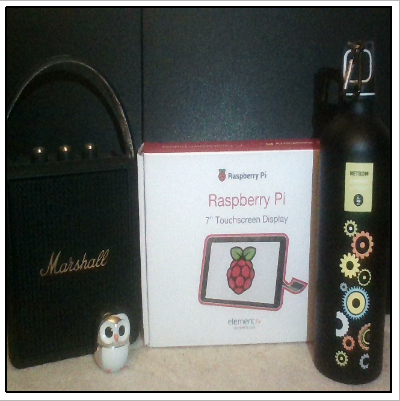
\includegraphics[width=0.45\textwidth, height=0.45\textwidth]{resources/Empty_4.png}
	\caption{Empty Filter Result}
\end{figure}

\subsection{Box Filter}

Also known as box blur, this filters inherent result is a diffuse copy of the original. This effect is
achieved through averaging the pixel neighborhood situated under the kernel. A basic 3x3 implementation
of the convolution mask \cite{ispBook}
\begin{equation}
	h = 1/9
	\begin{bmatrix}
		1 & 1 & 1 \\
		1 & 1 & 1 \\
		1 & 1 & 1 \\
	\end{bmatrix}
\end{equation}

The kernel can be generalized as \cite{opencvImproc}
\begin{equation}
	\label{eq:boxFilterFormula}
	h = \alpha
	\begin{bmatrix}
		1 & 1 & 1 & \dots & 1 \\
		1 & 1 & 1 & \dots & 1 \\
		\dots                 \\
		1 & 1 & 1 & \dots & 1 \\
	\end{bmatrix}
	\text{, where }
	\alpha =
	\begin{cases}
		1 / width * height & \text{, if normalized} \\
		1                  & \text{, otherwise}     \\
	\end{cases}
\end{equation}

OpenCV provides the implementation of \cref{eq:boxFilterFormula} in the form of the \verb|boxFilter| function.
The parameters provided to it are the kernel width and height, both of which can be set independently. The
result is a basic smoothing tool that accounts for the desired blur axis.

\begin{figure}[H]
	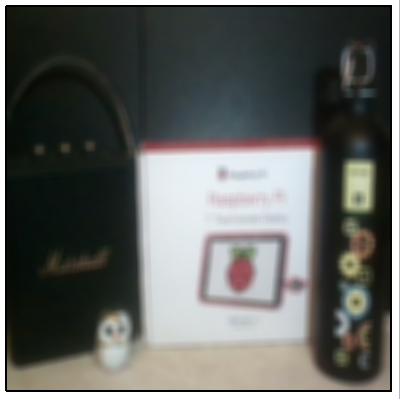
\includegraphics[width=0.45\textwidth, height=0.45\textwidth]{resources/Box_2.png}
	\caption{Box Filter Result}
\end{figure}

\subsection{Median Filter}

Similar to the box filter, median blurring also provides smoothing, however, it does so by replacing the
current pixel value with the median value inside its neighborhood. This is done in order to attenuate points
with intensity greatly different from those around it, points that would otherwise disproportionately affect
any other kind of smoothing operation. Those elements, formally known as ``salt and pepper`` noise have the
potential of hindering the functionality of other operators, so the median filter is an essential step in
ensuring image quality. \cite{fipBerkley}

It can be observed that for certain image functions \(f_1\) and \(f_2\), the following is true:
\[median(f_1(x, y) + f_2(x, y)) \neq median(f_1(x, y) + f_2(x, y))\]
For this reason, it can be concluded that the median filter is non-linear. In addition, due to the lack of
possibility for streamlining the finding of the median value, this smoothing technique is significantly more
computationally expensive than other methods, reason for which the kernel size must be significantly lower.

This is another filter provided in the image processing module, by the \verb|medianBlur| function, and is
solely characterized by the kernel size - parameter with little flexibility, due to the aforementioned
computational limitations.

\begin{figure}[H]
	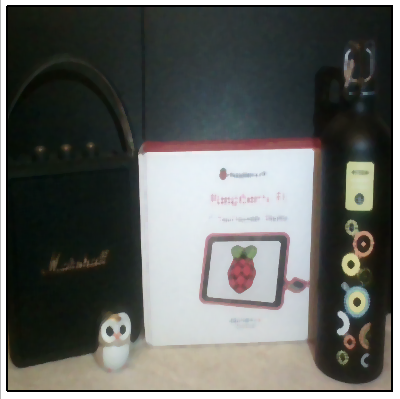
\includegraphics[width=0.45\textwidth, height=0.45\textwidth]{resources/Median_2.png}
	\caption{Median Filter Result}
\end{figure}

\subsection{Erode Filter}

Erosion is a ``morphological expression`` defined by a set of pixels \(A\) and a ``structuring element \(B\) \cite{dipBook}
as \[A \ominus B = \{z | (B)_z \subseteq A\}\] and refers to the notion that
``the erosion of \(A\) by \(B\) is the set of all points \(z\) such that \(B\), translated by z, is contained
in A``. \cite{dipBook}

In practice, as provided by the \verb|erode| function, the computation of the erosion is done by finding a
local minimum in each kernel, provided by a structuring element. \cite{opencvImproc}
\[erode(x, y) = \min\limits_{(x', y'): element(x', y') \neq 0} f(x + x', y + y')\]
Although an entire structuring element can be given as a parameter, for the purpose of this application only
the diameter of a square structuring element can be provided.

\begin{figure}[H]
	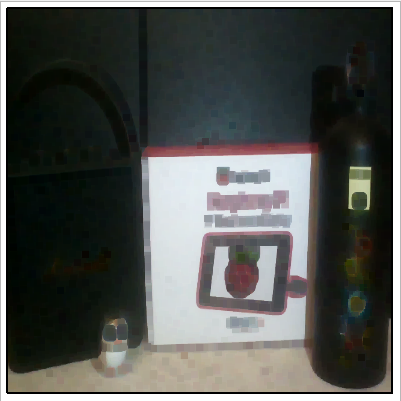
\includegraphics[width=0.45\textwidth, height=0.45\textwidth]{resources/Erode_2.png}
	\caption{Erode Filter Result}
\end{figure}

\subsection{Dilate Filter}

The dilation expression directly opposes the erosion, being defined on the same set of pixels \(A\) and
structuring element \(B\) \cite{dipBook} as
\[A \oplus B = \{z | (\hat{B}) \cap A \neq \emptyset\}\]

Also provided by OpenCV via the \verb|dilate| function, it achieves the opposite effect to the erosion,
computing instead the maximum value within the given structuring element and providing it to the current
pixel. \cite{opencvImproc}
\[dilate(x, y) = \max\limits_{(x', y'): element(x', y') \neq 0} f(x + x', y + y')\]
Also similar to the erode filter, dilation permits as a parameter the entire structuring element, however
only the kernel diameter is used.

\begin{figure}[H]
	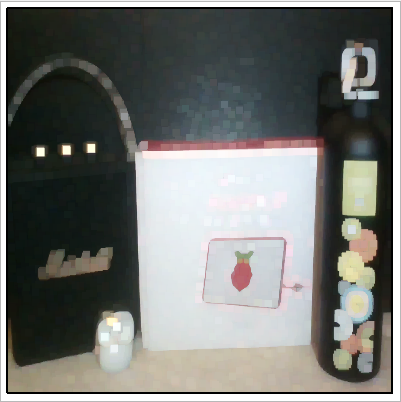
\includegraphics[width=0.45\textwidth, height=0.45\textwidth]{resources/Dilate_2.png}
	\caption{Dilate Filter Result}
\end{figure}

\subsection{Gaussian Filter}

The Gaussian filter, also called Gaussian blur, is a smoothing filter that based on the
Gaussian distribution function, defined in 2D space \cite{gaussian} by
\begin{equation}
	\label{eq:gaussianFormula}
	G(x, y) = {1\over\pi \sigma^2}{e^{(x^2 + y^2) / 2\sigma^2}}
\end{equation}

The curve defined in \cref{eq:gaussianFormula} can be visualized as:
\begin{figure}[H]
	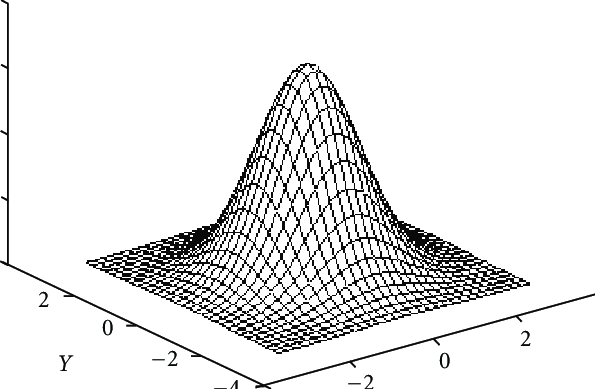
\includegraphics[width=0.30\textwidth, height=0.30\textwidth]{resources/Gaussian_Distribution.png}
	\caption{2D Gaussian distribution curve \cite{gaussian}}
\end{figure}

and approximated, in its normalized form, (for a \(\sigma\) value of \(1.4\)) with the integer kernel
\cite{gaussian}

\begin{equation}
	\label{eq:gaussianKernel}
	{1\over115}
	\begin{bmatrix}
		2 & 4  & 5  & 4  & 2 \\
		4 & 9  & 12 & 9  & 4 \\
		5 & 12 & 15 & 12 & 5 \\
		4 & 9  & 12 & 9  & 4 \\
		2 & 4  & 5  & 4  & 2 \\
	\end{bmatrix}
\end{equation}

OpenCV provides the implementation in the form of the \verb|GaussianBlur| function, defined by the size of
the Gaussian kernel applied, and the \(\sigma\) value for both the \(x\) and \(y\) axes. The associated
filter wrapper, however, only accounts for a single size parameter, that is distributed across both axes,
confiding the shape of the kernel in order to emphasize the effects of tweaking the \(\sigma\) value for
each direction.

\begin{figure}[H]
	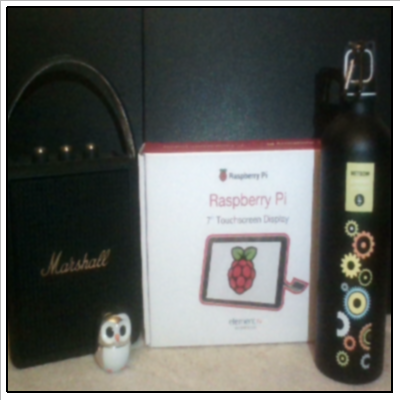
\includegraphics[width=0.45\textwidth, height=0.45\textwidth]{resources/Gaussian_2.png}
	\caption{Gaussian Filter Result}
\end{figure}

\subsection{Bilateral Correction}

As the last smoothing technique demonstrated in this application, bilateral filtering is also the most
complex, accounting not only for the neighborhood of each given pixel, but for the color disparity within
a given neighborhood. It can be represented \cite{bilateral} by
\begin{equation}
	\label{eq:bilateralFormula}
	k(x) = \int_{-\infty}^{\infty} c(\xi, x) s(f(\xi), f(x))
\end{equation}
where ``\(c(\xi, x)\) measures the geometric closeness`` and ``\(s(f(\xi), f(x))\) measures the photometric
similarity`` between point \(x\), denoting the neighborhood center, and point \(\xi\), representing a point
within the given neighborhood. \cite{bilateral}

The practical application of \cref{eq:bilateralFormula} is implemented by OpenCV within the
\verb|bilateralFilter| function, that takes into account the values for ``sigma color``, used to represent
the photometric similarity, and ``sigma space``, denoting the geometric closeness. It also accounts for the
kernel size, parameter that has the same functionality as ``sigma space``. \cite{opencvImproc}

Due to the use of color disparity, filter application leads to extended regions of similar color, regions that
do not intersect. The end result is a severely smoothed image, with great loss of minute detail. Object edges,
however, are entirely unaffected, causing for the shape of each macro element in the picture to be more easily
identifiable.

\begin{figure}[H]
	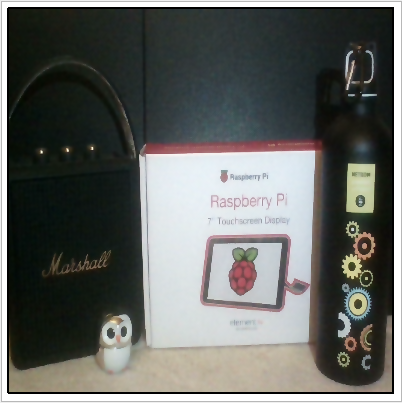
\includegraphics[width=0.45\textwidth, height=0.45\textwidth]{resources/Bilateral_2.png}
	\caption{Bilateral Filter Result}
\end{figure}

\subsection{Sobel Filter}

Another use for image filters is that of ``edge detection``. This refers to the application of operators
capable  of computing gradient differences in pixel intensity and color, leading to the minute outlining of
each distinct object present in the image.

One such implementation is provided by OpenCV via the \verb|Sobel| function, which computes ``the first,
second, third, or mixed image derivatives using an extended Sobel operator``. \cite{opencvImproc}
\begin{equation}
	\label{eq:sobelDerivatives}
	sobel(x, y) =
	{{\partial^{x_{order}+y_{order}}f(x, y)}\over{\partial x^{x_{order}} \partial y^{y_{order}}}}
\end{equation}

The practical implementation of \cref{eq:sobelDerivatives} is done through the ``Sobel operator``, an
extensible operator, used to compute the \(n-th\) order derivative on each axis. The 3x3 shape of the
first order derivative is represented for the \(x\) and \(y\) axes \cite{ispBook} as
\begin{equation}
	\label{eq:sobelOperators}
	h_x =
	\begin{bmatrix}
		-1 & 0 & 1 \\
		-2 & 0 & 2 \\
		-1 & 0 & 1 \\
	\end{bmatrix}
	,
	h_y =
	\begin{bmatrix}
		1  & 2  & 1  \\
		0  & 0  & 0  \\
		-1 & -2 & -1 \\
	\end{bmatrix}
\end{equation}

By computing the convolution of the initial image with the operators defined in \cref{eq:sobelOperators},
two separate images are obtained, each holding a partial gradient with respect to an axis:
\begin{equation}
	\label{eq:sobelResults}
	\begin{cases}
		G_x(x, y) = (h_x * f)(x, y) \\
		G_y(x, y) = (h_y * f)(x, y) \\
	\end{cases}
\end{equation}

Using the partial results, the final image, providing data on edges detected on both axes, can be computed
by calculating the ``magnitude`` of the pixel intensity for each location \cite{ispBook}
\begin{equation}
	\label{eq:sobelMagnitude}
	G(x, y) = \sqrt{G_x^2(x, y) + G_y^2(x, y)}
	\text{ or }
	G(x, y) = |G_x(x, y)| + |G_y(x, y)|
\end{equation}

The magnitude on each axis obtained with \cref{eq:sobelResults} can also be used to determine the angle
of the detected edge, through \cite{ispBook}
\begin{equation}
	\label{eq:sobelTheta}
	\tan(\theta) = {G_y\over{G_x}} \Rightarrow \theta = \arctan({G_y\over{G_x}})
\end{equation}

Implemented in the application, the wrapper for the Sobel filter takes several parameters, namely the size
and derivative order for the Sobel operator, a minimum value that the final image intensity can be scaled
up from, and a flag that determines weather the flat or directional version is computed and displayed.
The final result is scaled between the minimum value provided and a fixed maximum
\begin{equation}
	\label{eq:sobelScaling}
	f(x, y) = {f(x, y)(c_{max} - c_{min})\over{c_{max}}} + c_{min}
\end{equation}
where \(c_{min}\) denotes the specified minimum value, and \(c_{max}\) being either \(255\), in case of the flat
computation, where the magnitude is computed using the second approach from \cref{eq:sobelMagnitude}, or \(127\),
for the directional display, in which case the first approach for determining the pixel intensity provides
more accurate measurements. The value is different to the type of the \verb|cv::Mat| being changed from
unsigned integer to signed float when computing the magnitude, change that also provides greater accuracy when
computing the \(\theta\) angle value.

\begin{figure}[H]
	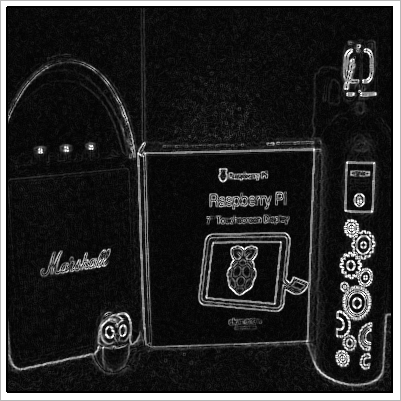
\includegraphics[width=0.45\textwidth, height=0.45\textwidth]{resources/Sobel_2.png}
	\caption{Sobel Filter Result - Non-directional}
\end{figure}

For the case of the non-directional edge detection, the image can be displayed once each pixel intensity is
computed. However, if the directional approach is desired, each color channel in the resulting image is used
to encode the angle as
\begin{equation}
	\label{eq:sobelRGB}
	\begin{cases}
		R = {1 - \cos(\theta)}           \\
		G = {1 - \cos(\theta + \varphi)} \\
		B = {1 - \cos(\theta - \varphi)} \\
	\end{cases}
\end{equation}
where the phase \(\phi\) can be adjusted in order to increase or decrease the range of colors available, and
is set to \(2\pi\over3\), in order to map the greatest possible range.

\begin{figure}[H]
	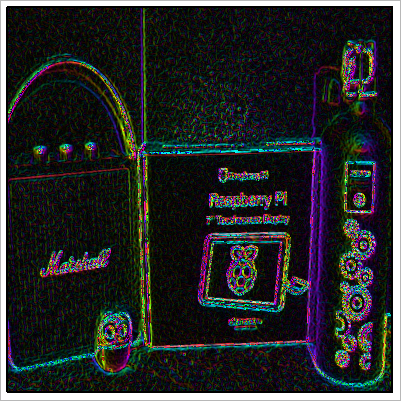
\includegraphics[width=0.45\textwidth, height=0.45\textwidth]{resources/Sobel_6.png}
	\caption{Sobel Filter Result - Directional}
\end{figure}

In this case, maximizing the lower intensity boundary results in the enhancement of the object shapes within
the image, and creates an effect similar to that of a depth map.

\begin{figure}[H]
	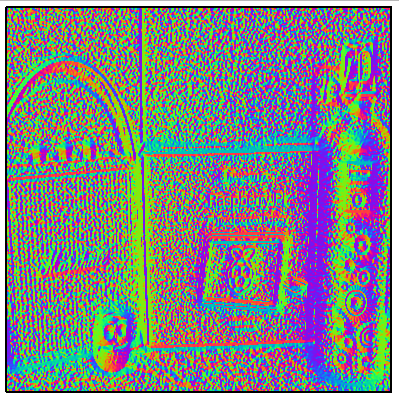
\includegraphics[width=0.45\textwidth, height=0.45\textwidth]{resources/Sobel_4.png}
	\caption{Sobel Filter Result - Directional Maximised}
\end{figure}

\subsection{Canny Filter}

The Canny approach to edge detection takes into account three criteria in order to optimize result quality
applied on images ``corrupted by white noise``. Those are ``detection``, referring to edge importance,
``localization``, referring to the distance between an edge and the position where it is detected, and the
``one response criterion``, referring to the removal of multiple hits for the same edge. This leads to the
resulting image pixels having only two possible states: edge pixels, encoded with an intensity of \(255\), and
non-edge pixels, encoded as 0s.

OpenCV provides the \verb|Canny| function, that achieves this result through the use of the Sobel operator
in order to detect edge intensities, and two parameters, a low threshold and a high threshold, used to
determine the weather a given pixel is part of an edge or not. After the Sobel operator is applied
elements with values above the high threshold are considered part of ``strong edges``, while the pixels with
magnitude under the low threshold are classified as not being part of an edge. For all intensities in between
those values, the aforementioned criteria are applied in order to determine a category.

The application allows for the tweaking of each threshold, leading to a more accurate edge detector, due to
the noise resistance being adjustable. It is specifically useful for situations in which an initial smoothing
step is undesirable or computationally expensive.

\begin{figure}[H]
	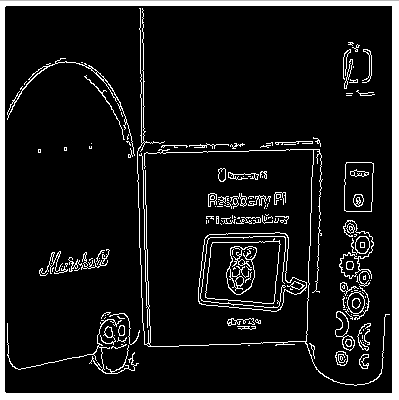
\includegraphics[width=0.45\textwidth, height=0.45\textwidth]{resources/Canny_2.png}
	\caption{Canny Filter Result}
\end{figure}

\subsection{Emboss Filter}

The aforementioned Sobel operator is able to detect an edge based only on the \(x\) and \(y\) axis, going from
top to bottom and right to left, other kernels can be used in order to provide directional data within the end
result. Such a kernel is the ``Prewitt operator``, a permutation of which is used for the purposes of this
application \cite{dipBook}
\begin{equation}
	\mathop{
		\begin{bmatrix}
			-1 & 0 & 1 \\
			-1 & 0 & 1 \\
			-1 & 0 & 1 \\
		\end{bmatrix}
	}_{\textstyle \text{Prewitt operator}}
	\Rightarrow
	\mathop{
		\begin{bmatrix}
			-1 & -1 & 0 \\
			-1 & 0  & 1 \\
			0  & 1  & 1 \\
		\end{bmatrix}
	}_{\textstyle \text{Permutation}}
\end{equation}

The generated operator can be used to detect transitions on a 45\textdegree offset from the main axis. This
kernel can also be rotated, either by 45\textdegree or 90\textdegree, in order to achieve different results.

For use in this application, each kernel rotation is manually generated, with the sole parameter of the
filter wrapper being the rotational step of the initial kernel, with each increment denoting a 90\textdegree
rotation of the initial operator. After the convolution is computed, a fixed base value is added to the
result, in order to flatten the output. The final image will represent a gray-scale version of the input,
with intensity peaks where edges were detected, a result that resembles an embossed sheet of metal.

\begin{figure}[H]
	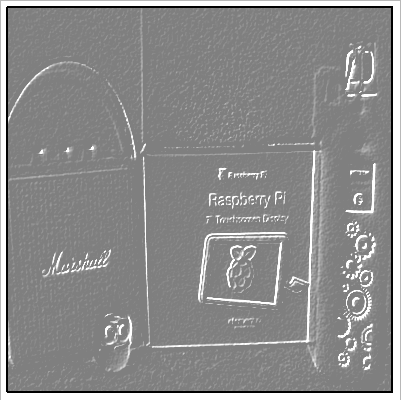
\includegraphics[width=0.45\textwidth, height=0.45\textwidth]{resources/Emboss_2.png}
	\caption{Emboss Filter Result}
\end{figure}

\subsection{Lens Distortion}

A fairly common occurrence in photography, lens distortion appears as a result of light rays being diverged
by complex lens arrays. It is defined by the curvature appeared in the image of lines that are, in reality,
straight. For this reason it is also referred to as ``curvilinear`` distortion The phenomenon is directly
linked to lens curvature and focal length, and ,depending on those factors, several types of aberrations
can be noticed. \cite{lensImages}
\begin{figure}[H]
	\label{fig:distortionTypes}
	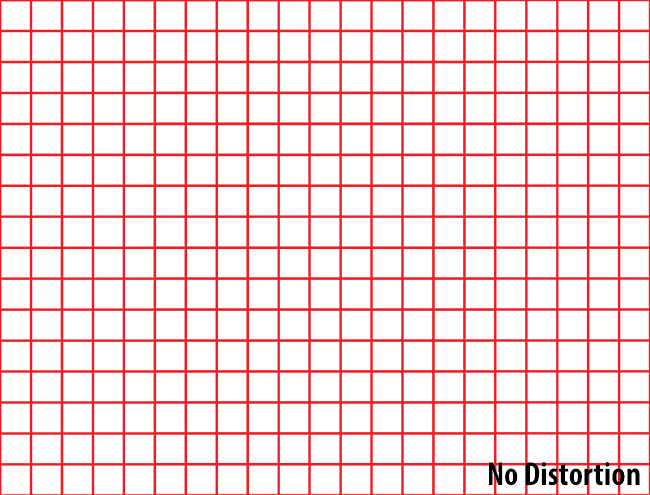
\includegraphics[width=0.2\textwidth, height=0.2\textwidth]{resources/No-Distortion.png}
	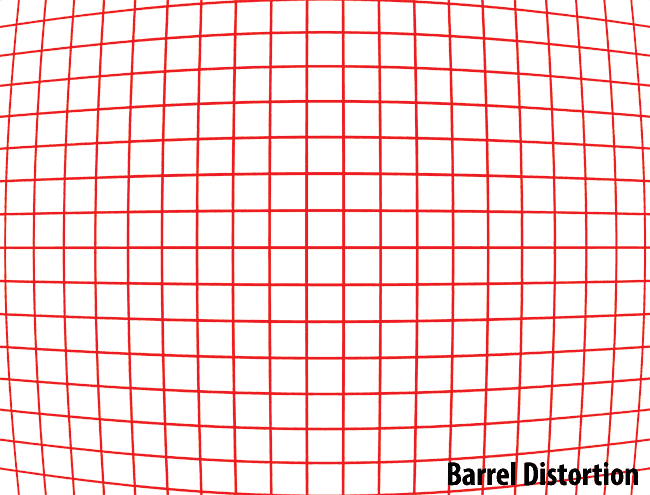
\includegraphics[width=0.2\textwidth, height=0.2\textwidth]{resources/Barrel-Distortion.png}
	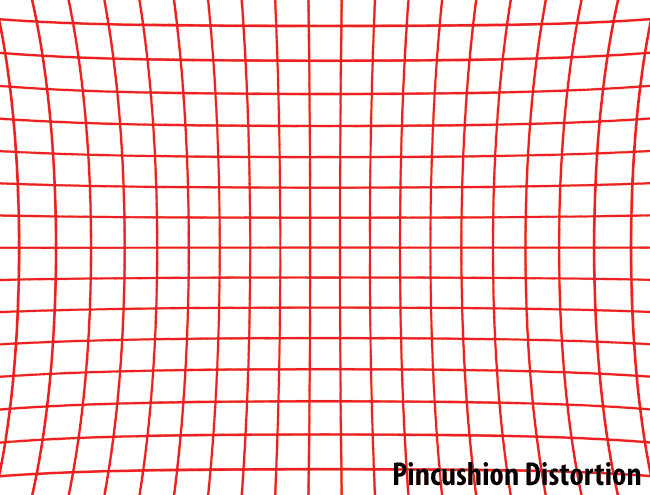
\includegraphics[width=0.2\textwidth, height=0.2\textwidth]{resources/Pincushion-Distortion.png}
	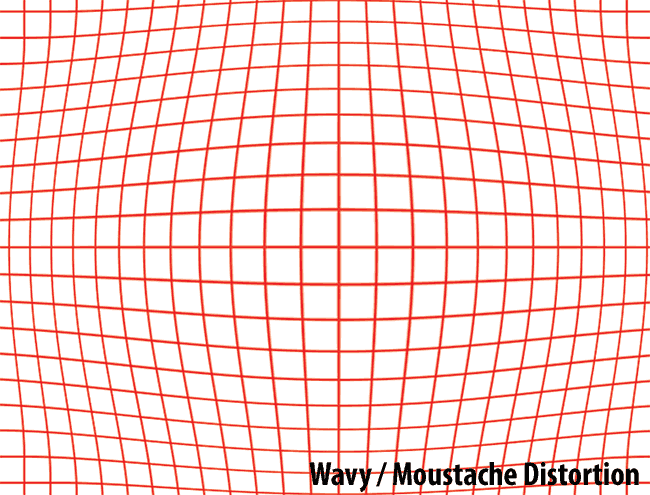
\includegraphics[width=0.2\textwidth, height=0.2\textwidth]{resources/Wavy-Moustache-Distortion.png}
	\caption{Distortion types \cite{lensImages}}
\end{figure}

The nomenclature used for each distortion type in \cref{fig:distortionTypes} is related to the aspect of each
aberration. ``Barrel distortion`` refers to the outwards curvature of the lines, defining the shape of a
barrel. In the case of ``Pincushion distortion``, the lines curve inwards, with the center being unaffected,
thus resembling a pincushion. ``Wave distortion`` represents a combination of the aforementioned aberrations,
with lines being curved outwards towards the center of distortion, and inwards around the edges and corners.
For this reason, wave distortion is significantly more difficult to account for or later correct.

Due to the physical nature of the distortion, with light rays hitting the image sensor in places that do not
correspond with the real-life picture, the proposed solution does not affect the intensity values of each
pixel, but modifies their geometric location. A general re-mapping implementation \cite{lensFromula} is
\begin{equation}
	\label{eq:lensFormula}
	\begin{cases}
		x_u = x_d(1 + \lambda_1r_d^2 + \lambda_2r_d^4 + \dots) \\
		y_u = y_d(1 + \lambda_1r_d^2 + \lambda_2r_d^4 + \dots) \\
	\end{cases}
\end{equation}
where \(x_d\) and \(y_d\) refer to the initial, distorted coordinates, \(x_u\) and \(y_u\) refer to the
undistorted output, and \(r_d\) refers to the distance of the current point from the center coordinates,
usually \((0, 0)\), with \(r_d = \sqrt((x_d - x_0)^2 + (y_d - y_0)^2)\).

For efficient computation and usability, only the first \(\lambda\) parameter is computed using \cite{lensStack}
\begin{equation}
	\label{eq:lensLambda}
	\lambda_1 = (\sin({{\pi r_d}\over{2 r_{max}}}))^{d_c}
\end{equation}
with \(r_{max}\) denoting the maximum radius around the center that is affected by the algorithm, and \(d_c\)
representing the distortion coefficient.

The filter is capable of inducing both barrel and pincushion distortion, with the differentiation being done
through the distortion coefficient. For positive values, barrel distortion will be applied,

\begin{figure}[H]
	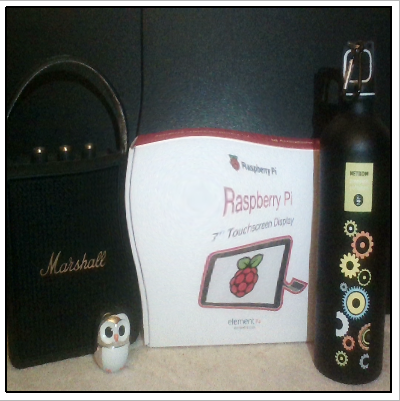
\includegraphics[width=0.45\textwidth, height=0.45\textwidth]{resources/Lens_2.png}
	\caption{Lens Filter Result - Barell Distortion}
\end{figure}

and for negative, pincushion aberration will be created.

\begin{figure}[H]
	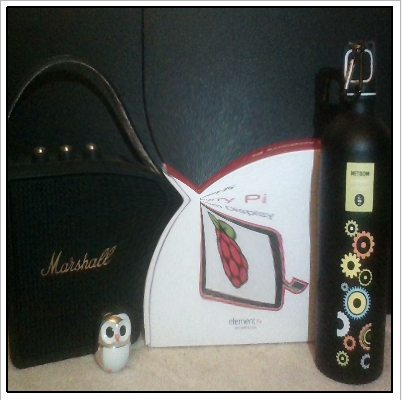
\includegraphics[width=0.45\textwidth, height=0.45\textwidth]{resources/Lens_4.png}
	\caption{Lens Filter Result - Pincushion Distortion}
\end{figure}

The magnitude of the coefficient represents the impact that the filter
will have on the end result. The wrapper takes as parameters the maximum distortion radius and the distortion
coefficient. It would also be possible to implement parameters for changing the position of the distortion
center, however, due to the user interface implementation, it is not required.

\section{User Interface}

Based on the QtFramework \verb|QWidget| system, this library provides the input and display management system
for the entire application. Its functionality covers both user input, as well as camera input obtained via
the \verb|VideoCapture| interface. Each frame has to be captured, processed, converted to a Qt compatible
format and displayed.

After a given frame is captured off of the systems default camera, it is firstly resized in order to match the
viewports height and with, such that it is compatible with the region of interest. Afterwards, each selected
filter is applied on the image, which is still under the shape of a \verb|cv::Mat|. Following this process,
the result is then converted into a \verb|QPixmap|, such that it is compatible with the rest of the UI
elements. The conversion takes into account the amount of channels in the captured image and outputs to a
single RGBA format. It is then displayed to the user in the viewport, which is represented by a
\verb|QGraphicsView|, encasing a \verb|QGraphicsScene|. \cite{qtConvert, qtDoc}

The entire interface layout cab be broken down into two main components - the viewport displaying the most
recently processed frame, and the control panel, used to modify the type and amount of filters applied, as
well as parameters for each. Those elements are, in turn, comprised of other dedicated submodules, leading
to a tree of encapsulated widgets, with the following layout.

\begin{figure}[H]
	\label{fig:uiSchema}
	\begin{tikzpicture}[%
			grow via three points={one child at (0.5,-0.7) and
					two children at (0.5,-0.7) and (0.5,-1.4)},
			edge from parent path={(\tikzparentnode.south) |- (\tikzchildnode.west)}]
		\node {Window}
		child { node {Viewport}
				child { node {Scene}
						child {node {Pixmap}}
						child {node {Region of interest}
								child{node {Anchor}}
							}
					}
			}
		child [missing] {}
		child [missing] {}
		child [missing] {}
		child [missing] {}
		child { node {Control Panel}
				child{node {Miscellaneous}
						child{node {Toggle Freeze}}
						child{node {Toggle Selection}}
					}
				child [missing] {}
				child [missing] {}
				child{node {Layer Management}
						child{node {Add Layer}}
						child{node {Delete Layer}}
						child{node {Move Layer Up}}
						child{node {Move Layer Down}}
					}
				child [missing] {}
				child [missing] {}
				child [missing] {}
				child [missing] {}
				child{node {Filter Selection}
						child{node {Filter Information}}
						child{node {Filter Parameters}}
					}
			};
	\end{tikzpicture}
	\caption{Widget nesting diagram}
\end{figure}

After each element described in \cref{fig:uiSchema} is implemented and placed into its parent layout, with the
following end result.

\begin{figure}[H]
	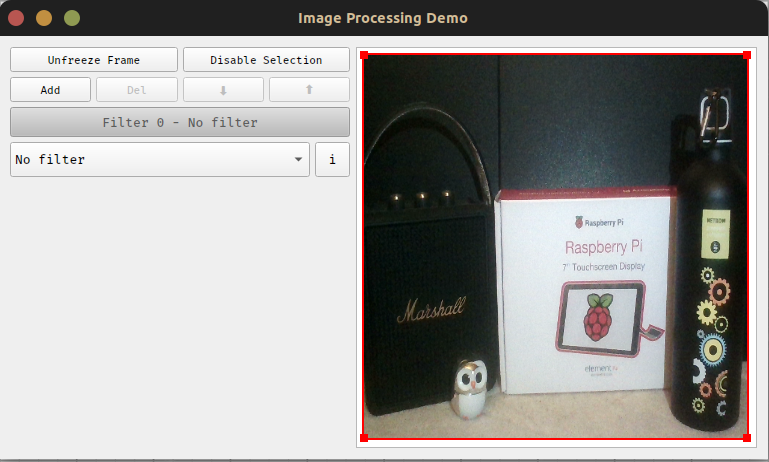
\includegraphics[width=0.9\textwidth, height=0.45\textwidth]{resources/Empty_1.png}
	\caption{User Interface Overview}
\end{figure}

\subsection{Region of Interest}

The region of interest represents the portion of the captured frame that is affected by any given filter. Its
primary use is to confine a filter to a subset of the original image, in order to create a context for
comparing and contrasting the before and after displays of the same set of features.

It is implemented as a child of the \verb|QGraphicsItem| class, due to its inherent properties, mainly being
resizable and movable withing the scene. This is achieved through opperating on the items ``bounding
rectangle``. \cite{qtDoc}

The resizing of a region of interest is done through the anchors present in each corner of its parents
bounding rectangle. The anchors are also inherited from \verb|QGraphicsItem|, and can be moved only within
the confines of the scene. Each anchor also affects the position of its neighbors, such that the region of
interest is always rectangular. The regions bounding rectangle is always drawn in between the top-left and
bottom-right anchors, in order to ensure the expected behavior if two anchors were to overlap.

\begin{figure}[H]
	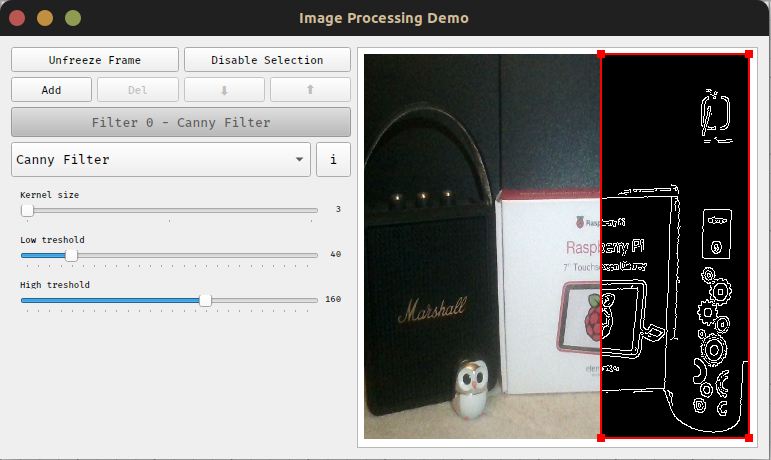
\includegraphics[width=0.9\textwidth, height=0.45\textwidth]{resources/Roi_1.png}
	\caption{Resized Region of Interest}
\end{figure}

In case of a region of interest smaller than the bounds of the scene, it can be moved around the scene, as
long as its anchor points remain within bounds. This is done in order to preserve the integrity of the applied
filters.

\begin{figure}[H]
	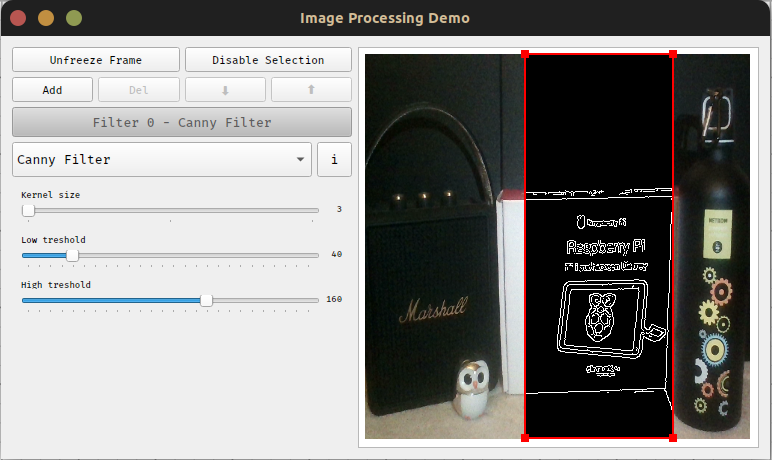
\includegraphics[width=0.9\textwidth, height=0.45\textwidth]{resources/Roi_2.png}
	\caption{Moved Region of Interest}
\end{figure}

\subsection{Layer system}

In order to provide the experience of combining different filters, such that the interaction between them can
be observed and studied, the layer system allows for the sequential application of several filters on any one
frame. Each layer operates within its own region of interest, which has to be accounted for when applying the
desired filters.

The main features of the \verb|Layer| class are the \verb|GenericFilterWrapper*| array, holding exactly one
of each type of filter available, and the \verb|applyFilter| function, that first maps the region of interest
onto the input image, applies the filter currently selected onto the subsection, and copies the selection back
to the original, keeping the region parameters unchanged.

It can be used to gauge the ways each filter can affect another, such as the case for the Sobel and Dilate
filters. If the Sobel operator is applied first, the result will be further enhanced by the Dilate filter
picking up each edge pixel as a local maximum and spreading its intensity to the neighboring pixels:

\begin{figure}[H]
	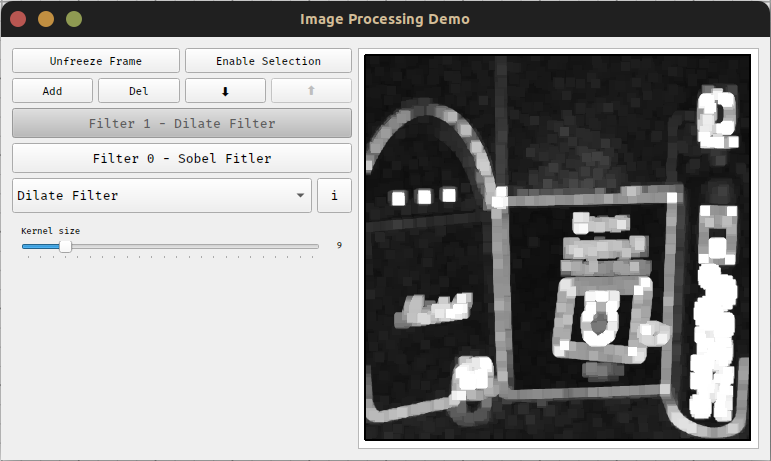
\includegraphics[width=0.9\textwidth, height=0.45\textwidth]{resources/Layers_1.png}
	\caption{Dilate filter applied on top of Sobel}
\end{figure}

To contrast, if the Dilate is applied first, then the entire image will be segmented into chunks of similar
or identical color, leading to the edges determined by the Sobel operator to be jagged, following the color
difference between any neighboring chunks:

\begin{figure}[H]
	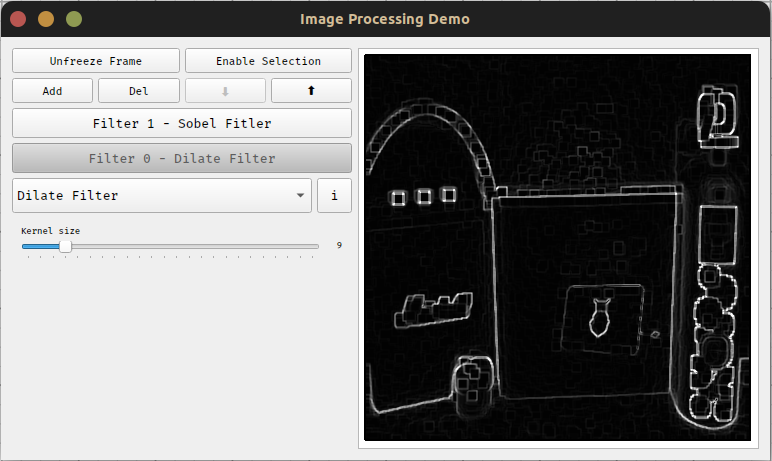
\includegraphics[width=0.9\textwidth, height=0.45\textwidth]{resources/Layers_2.png}
	\caption{Sobel filter applied on top of Dilate}
\end{figure}

Another use of this system is the combination of smoothing operators, targeted on noise removal, with more
visually impactful filters, such as edge detection or lens distortion. The current application capacity is
at three filters, due to the computational strain each additional filter produces.

\begin{figure}[H]
	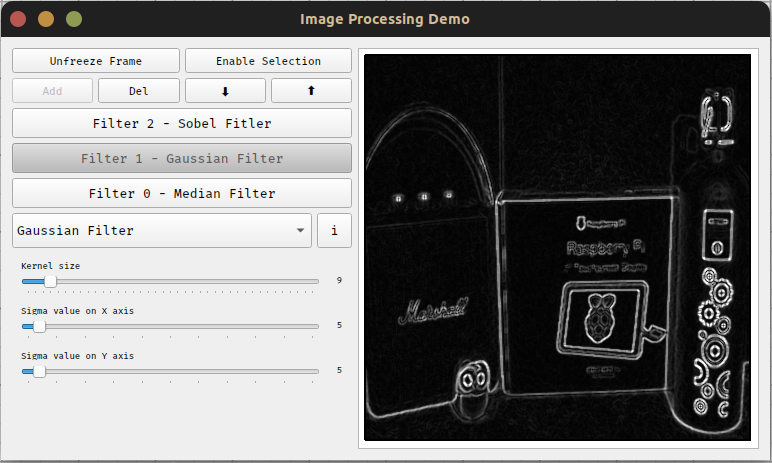
\includegraphics[width=0.9\textwidth, height=0.45\textwidth]{resources/Layers_3.png}
	\caption{Smoothing filters applied before edge detection}
\end{figure}

\subsection{Signals and Slots}

Like many other user interface frameworks, Qt also provides event-based communication, through the use of
``signals and ``slots``. Signals are present on event senders, such as timers and buttons, and dictate the
type of event that is being triggered. Slots are implemented on the side that needs to respond to an event,
such as a value update of filter swap. The link between those function categories is done through the
\verb|connect| function, that takes as inputs two objects, a signal acting on the first object and a slot
comprising the second, slot that can be expressed a lambda function if the need arises. \cite{qtDoc}

Signals and slots are used throughout the entire user interface in order to communicate state changes and
required updates, most important of which is the frame change functionality. Tied to the \verb|timeout|
signal of a \verb|QTimer|, the \verb|Update| slot of the main window is responsible for the entire process
of accessing the current frame, applying all the required filters and displaying the result in the scene.
This function is triggered every \(33 ms\), leading to a potential frame rate of \(30 FPS\).

The other main functionality of this communication system is to control the aforementioned layers, regions
of interest and filter parameters. Achieved through the use of buttons, sliders and combo boxes, this
functionality is managed through the control panel, or sidebar.

\subsection{Control panel}

The sidebar is the main user interaction hub for the application. It is comprised of several sub-layouts,
each encompassing interactable widgets that serve a common purpose. Those layouts are, in order:
miscellaneous, layer control, layer select, filter select, parameter tweak.

The miscellaneous sections is comprised of two button, each responsible for toggling a different feature of
the application. The \verb|Toggle Freezeframe| button was added in order to provide the means of alleviating
computational strain, in case the desired filter combination proves to be too computationally expensive for
the given system to handle at a manageable frame rate. It will stop the capturing of a new frame, allowing for
tweaks to be done on a constant input stream, thus leading to a more consistent comparison. The
\verb|Toggle Selection| button allows for the removal of any layer selection, consequence of which is the
locking of the region of interest and the removal of its potentially distracting outline.

Four buttons comprise the layer control layout, two of which are used for adding or removing a layer, and  the
other two for changing layer position relative to its neighbors. Similar to other image manipulation software,
the layer order is bottom-up, with the lowest filter in the stack being applied first, and the top one last.

\begin{figure}[H]
	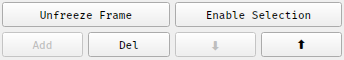
\includegraphics[width=0.8\textwidth, height=0.2\textwidth]{resources/Buttons_Misc.png}
	\caption{Miscellaneous and Layer control layout}
\end{figure}

The third section provides functionality for selecting each layer, one at a time. The layer currently selected
is highlighted and it cannot be selected again. When selecting a filter, its region of interest becomes active,
meaning that it can be interacted with for movement and resizing. The layer order is in accordance with the
order in which they are applied on the current frame, and it is updated whenever a layer is added, removed
or changes position.

\begin{figure}[H]
	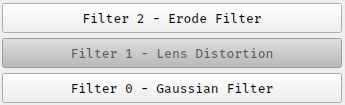
\includegraphics[width=0.8\textwidth, height=0.3\textwidth]{resources/Buttons_Layers.png}
	\caption{Layer select layout}
\end{figure}

The aforementioned layouts are entirely comprised of \verb|Buttons|, a child class of the \verb|QPushButton|
class. Each functionality is tied to the \verb|QPushButton::clicked| signal through a lambda function providing
the slot implementation. \cite{qtDoc}

For selecting the filter applied on the current layer, a \verb|QComboBox| is populated with the data relevant
to each filter wrapper contained within the layer implementation. It is built at every layer change, in order
to set its value to the filter present on the newly selected layer. After a filter is selected, both the
viewport and the other controls are updated with the current wrapper parameters. The other component of this
layout is the \verb|Information| button, whose \verb|QPushButtonPressed| signal is tied to a lambda function
that can show a \verb|QToolTip| on the current cursor position, tool-tip that provides information about the
filter and each of its parameters. \cite{qtDoc}

\begin{figure}[H]
	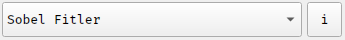
\includegraphics[width=0.8\textwidth, height=0.09\textwidth]{resources/Buttons_Selector.png}
	\caption{Filter select layout}
\end{figure}

The final component of the control panel is specific for each filter, and that is the parameter tweaking
sliders, each of which is based on the \verb|QSlider| parent class. All sliders are built based off of the
structure presented in \cref{code:parameterConfig}, and is layer independent. This means that, if the same
filter is applied from two different layers, each filter will have its private set of parameters modified
at a given time. The slider steps and boundaries were chosen in accordance to the OpenCV specifications,
in order to not run into incompatibility issues, and with great consideration towards the set of measurements
done in order to observe filter latency.

\begin{figure}[H]
	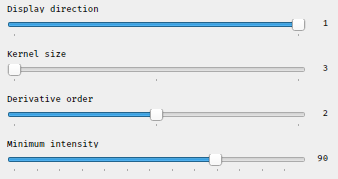
\includegraphics[width=0.8\textwidth, height=0.5\textwidth]{resources/Buttons_Sliders.png}
	\caption{Filter parameters layout}
\end{figure}



